\section{Le Méta-Modèle Entity}\label{sub:ent}
Les Entity permettent de simplifier la gestion des données au niveau d'une application, mais aussi de faciliter la sauvegarde en base de données. Plus concrètement, ces Entity nous permettent de prendre en charge la persistance des données de notre application dans une ou plusieurs sources de données, tout en gardant les relations entre celles-ci. Ces composants établissent donc la relation entre notre application et notre bases de données.
Un méta-modèle Entity a été établie par Obeo afin de représenter la structure des Entity qui vont définir la couche métier de notre application. La figure \ref{fig:ent}  montre le méta-modèle Entity simplifié.

\begin{figure}[htb]
  \centering
  
\includegraphics[scale=.4]{img/Entity.eps}
  \caption{Méta-modèle Entity}
  \label{fig:ent}
\end{figure}

Tout modèle conforme au métamodèle "Entity" peut être constitué de plusieurs de plusieurs Bloques (blocks). Chaque bloque se compose de plusieurs Entity. Celle-ci possède un ou plusieurs attributs, et peut référencer d'autres Entity. Un attribut peut avoir une métadonnée qui peut être constituée d'une ou plusieurs annotations.   

\subsection{Gestion des entités avec \kwplay{}}
Dans la plate-forme Play, tout le code métier est porté par les objets du modèle. Celui-ci contient les données persistantes, ce qui s'accordent parfaitement avec le concept d'\kwentity.  
On peut par exemple écrire le code suivant pour manipuler une entité "Personne" :\\
// Si on voulait récupérer toutes les personnes    \\
List<Personne> personnes = Personne.find("byName","Takfarinas").fetch();  \\
Personne p1 = Personne.findById(1);  // Récupérer la personne ayant l'id 1  \\
p1.firstName = "paul";  // Modification de l'entité  \\
p1.save(); // Mise à jour dans la base de données    
         

\subsection{Conception du modèle}
Nous avons employé la simple démarche suivante : pour chaque module Play on associe une entité. À ce stade, on en déduit facilement les attributs de chaque instance d'\verb+Entity+ et les instances \verb+Reference+ correspondant aux associations avec d'autres entités. \kwplay{} utilise des mécanismes d'annotation au sein de ses modèles. Ces annotations permettent notamment de donner des contraintes à des attributs. Nous avons facilement pris en compte ce concept en utilisant la classe \verb+Annotation+ mise à disposition dans les méta datas d'un \verb+Attribut+.\\
Nous avons élaboré un modèle d'entity de notre application conformément au méta-modèle que nous avons décris en dessus. Ce modèle est illustré par la figure \ref{fig:entMod} ci-dessous.

\begin{figure}[H]
  \centering
  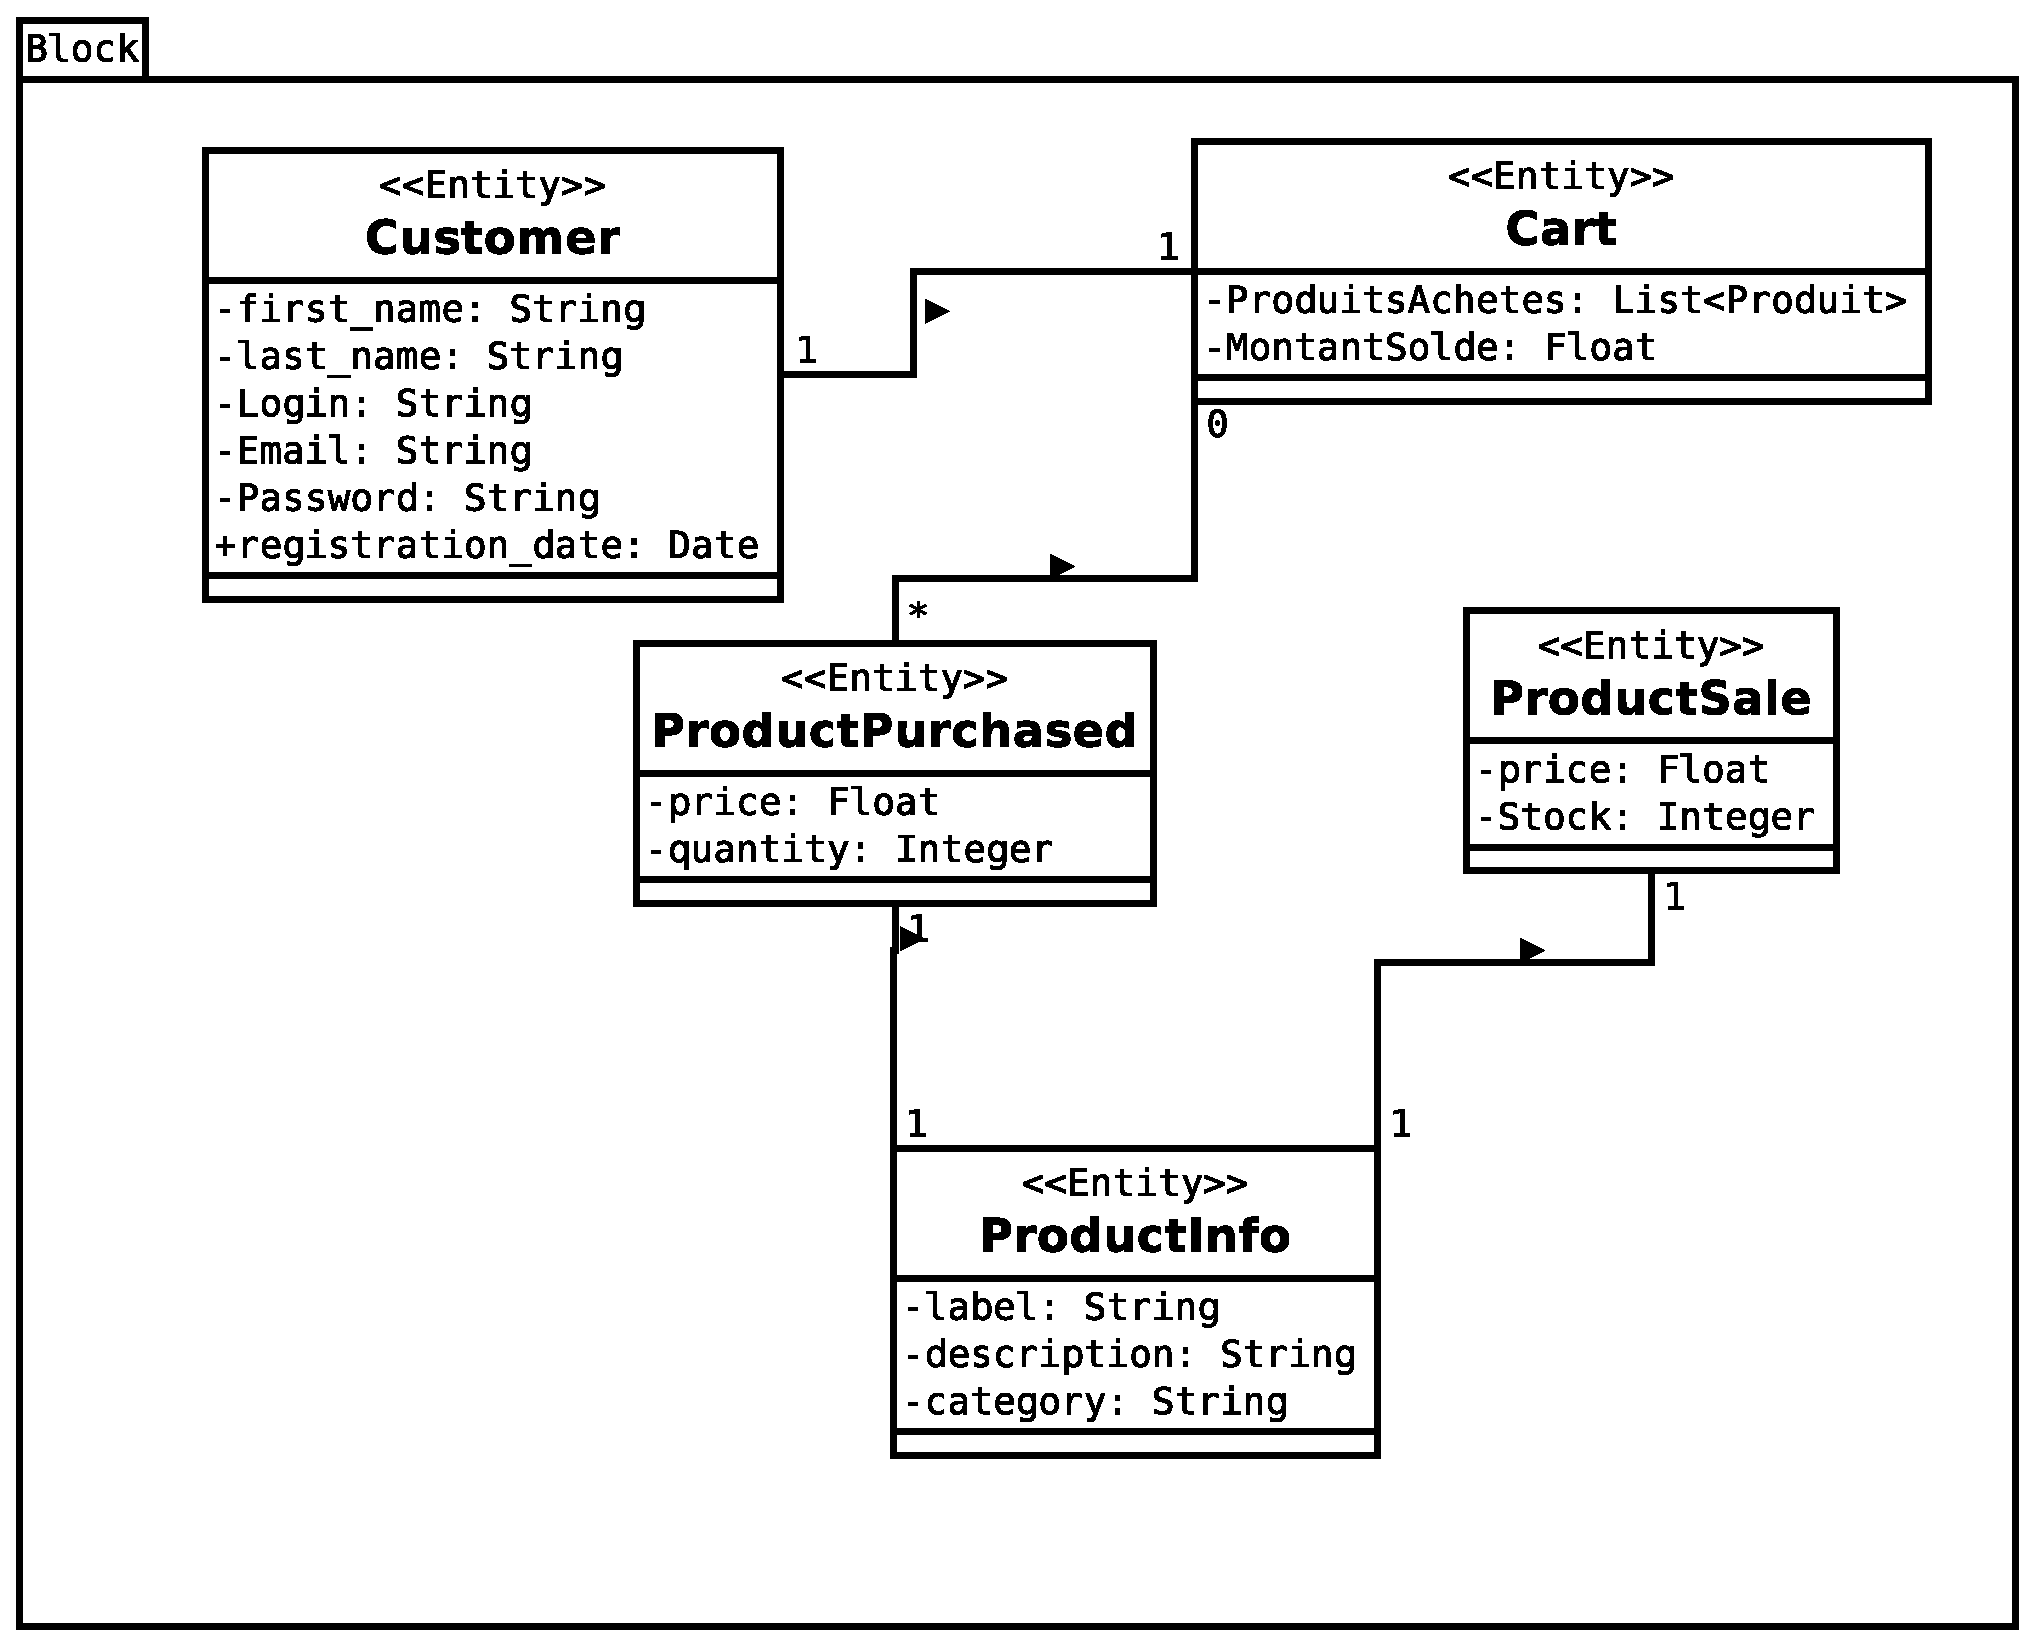
\includegraphics[scale=.4]{img/Entitymodel.eps}
  \caption{modèle Entity de l'application}
  \label{fig:entMod}
\end{figure}

Nous avons représenté un seul bloque dans notre modèle d'Entity qui va regrouper les Entity suivantes :  

\begin{itemize}
  \item[\textbullet] \textbf{Costumer} : Représente le client qui va faire l'achat sur la plate-forme
  \item[\textbullet] \textbf{ProductSale} : représente les produits mises en vente.
  \item[\textbullet]	\textbf{ProductPurchased} : représente les produits achetés par un client.
  \item[\textbullet] \textbf{ProductInfo} : contient les informations d'un produit.
  \item[\textbullet] \textbf{cart} : représente une carte de paiement reliant un client aux produits qu'il a acheté.
   
\end{itemize}






\clearpage



% LocalWords:  Entity framework Model
